\chapter{関連語句}
\section{ガボールフィルタ}
ガボールフィルタとは,画像を周波数領域でテクスチャ解析する方法のひとつ.
テクスチャ解析とは,粗い,滑らか,でこぼこなどの直感的な材質を,画素強度の空間的な変動の関数として定量化する試みのことである\cite{テクスチャ解析}.
テクスチャ解析する方法として,フーリエ変換がある.フーリエ変換では画像をいくつかのブロックに区切る必要があり,対象の境界も同時に検出するという問題に対して,結果が粗くなる.
周波数の不正確さと,位置の不正確さとの積には下限があり,それを最小にするのは「ガボール関数」である.\par
ガボール関数は,サルの一次視覚野にある単純細胞の受容野特性によく似ており,ガボール関数の正弦波や余弦波の傾きを変化させることで.この受容野特性をよく再現できる.
\begin{flushright}
    \cite[p.144]{認知心理学辞典}
\end{flushright}
\section{固有顔法}
固有顔(eigenface)とは,顔画像の認識において最も有名な手法のひとつ.
顔認識では,顔を構成する部品(目や鼻,口など)の形状や,配置から特徴点を抽出して認識に利用する.しかし,照明方向や,撮影距離,表情,顔の傾きなどで顔の見え方が変わる.これらを許容したうえで正しく顔認識するには,顔画像をパターンとして扱い,統計的パターン認識手法を適用する方法がある.
まず挙げられるのが,パターン間のマッチングを用いた方法である.この方法は最も簡単なパターン認識手法であるが,画像そのものをパターンとして扱った場合,パターンの次元が大きくなる.
この問題を解決する方法として提案されたのが,固有顔である.固有顔は主成分分析によりパターンを情報圧縮し,顔画像の識別に利用している.
数枚の画像に対して,各画像から平均ベクトルを引いた集合に対して,固有値を求める.この時の固有ベクトルを固有顔と呼ぶ.\par
\hfill\cite{顔画像からの個人識別}
\section{オプティカルフロー}
視覚におけるオプティカルフローとは,前方へ移動するときの,後ろへ流れる背景のことである.
このオプティカルフローには2種類の特性があり,身体が対象へ直線的な移動時に起きる「放射状オプティカルフロー」,身体が回るときに起きる「回転性のオプティカルフロー」が存在する\cite[p.679]{人間の運動学}.\par
また,動画像処理におけるオプティカルフローとは,動画像中の物体の動きを検出して,速度をべクトルで表示する手法を指す.
フロー推定方法としてブロックマッチング法を取り上げる.ブロックマッチング法は,画像のある大きさのブロックで分割し,次フレームにおける注目ブロックとの類似度が最も大きいブロックを検出する手法である\cite{オプティカルフローを用いた画像中の野鳥検出}.
\newpage
\section{ストラクチャ フロム モーション(SfM: Structure from Motion)}
\begin{wrapfigure}{r}[0mm]{.3\textwidth}
    \centering
    \vspace{-.5cm}
    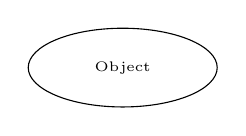
\begin{tikzpicture}
        \draw (0,0)circle(1.2 and 0.5)node{\tiny Object};
    \end{tikzpicture}
    % \vspace{-.5cm}
\end{wrapfigure}
SfM\footnote{以後,ストラクチャ フロム モーションをSfMと記す.}とは,一連の2次元イメージから,3次元シーンの構造を推定するプロセスを指す.
具体的には,ドローンによる空撮写真(2次元)から3次元のデータを得るときに用いられる.
ここでは,例として2つのビュー(カメラ)によるSfMを取り上げる.
カメラ1で読み取った画像(\texttt{img1})と,カメラ2で読み取った画像(\texttt{img2})の対応関係を抽出した後,カメラ1に対するカメラ2の姿勢を求める.
このときに,基礎行列を計算し,エピポーラ幾何を
